\chapter{Methodology and Implementation}

\section[Approach]{\textbf{Approach}}

\subsection{System Overview}

The methodology follows an event-driven architecture that connects wearable sensing, local fall prediction and verification, emergency escalation, ambulance tracking, hospital pre-notification, and dashboard-based monitoring in a layered workflow.

\subsection{Proposed System Architecture}

The EdgeCare Response platform follows a distributed architecture with clear separation of concerns connecting the wearable edge node to the cloud backend and user interface:

\begin{figure}[htb]
\centering
	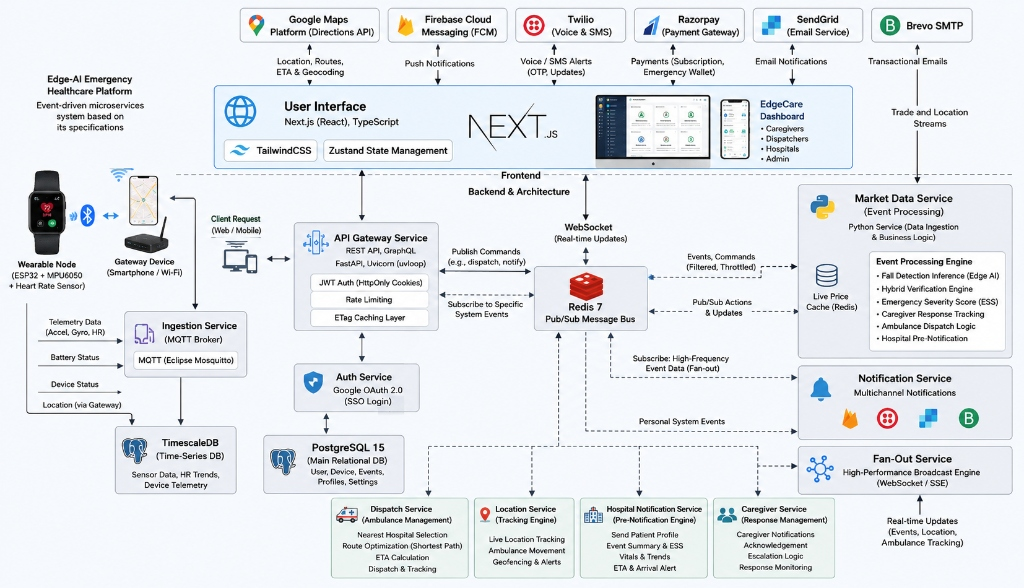
\includegraphics[width=\textwidth]{Figures/system_architecture.jpg}	
	\caption{Edge-AI Emergency Healthcare Platform System Architecture}
	\label{fig:system_architecture}
\end{figure}

The architecture comprises the following layers:
\begin{enumerate}
\item \textbf{Wearable Sensing Layer}: ESP32 with MPU6050 accelerometer, gyroscope, and heart-rate sensor.
\item \textbf{Gateway Layer}: Smartphone or Wi-Fi router for cloud synchronization and location services.
\item \textbf{Edge-AI Processing Layer}: TinyML model and physiological verification logic running on the ESP32.
\item \textbf{Cloud Services Layer}: Next.js backend, notification workflows, and severity assessment.
\item \textbf{User Interface Layer}: Web dashboard for caregivers, dispatchers, and hospitals.
\end{enumerate}

\subsection{Data Flow Architecture}

The data flow within the EdgeCare Response platform starts at the wearable sensor node and moves through the mobile gateway, API gateway, real-time message brokers, processing services, and target notification endpoints, as shown in Figure~\ref{fig:dataflow_architecture}.

\begin{figure}[htb]
\centering
	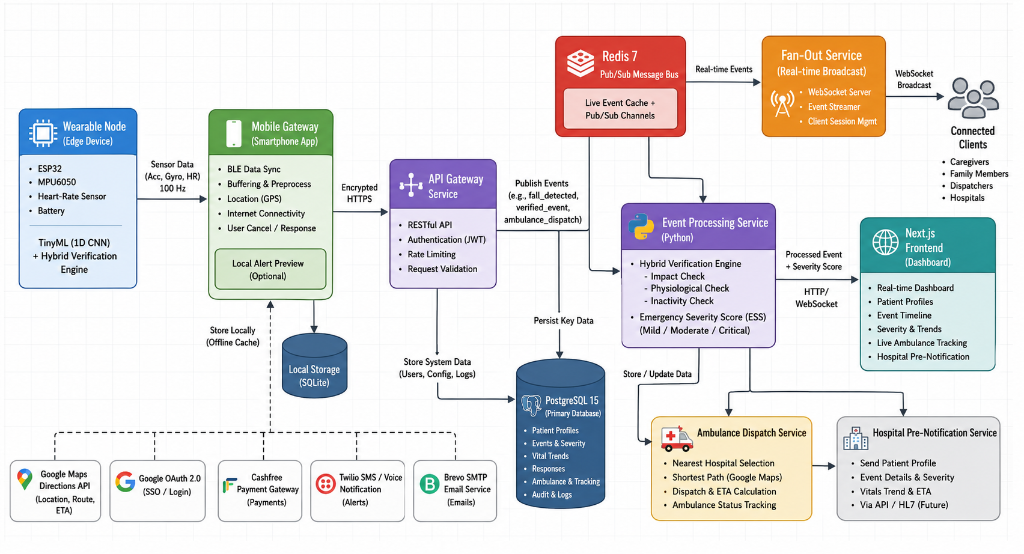
\includegraphics[width=\textwidth]{Figures/dataflow_architecture.png}	
	\caption{EdgeCare Response Platform Data Flow Architecture}
	\label{fig:dataflow_architecture}
\end{figure}

The primary data flows are:
\begin{enumerate}
\item \textbf{Sensor Data Sync}: Wearable Node (ESP32, MPU6050, Heart Rate Sensor) streams sensor data (Acc, Gyro, HR) at 100 Hz to the Mobile Gateway via Bluetooth Low Energy (BLE). On-device processing is performed using a TinyML (1D CNN) and Hybrid Verification Engine.
\item \textbf{Ingress \& Gateway}: The Mobile Gateway buffers the data, adds GPS location coordinates, and transmits it via encrypted HTTPS requests to the API Gateway Service (which handles RESTful APIs, JWT authentication, rate limiting, and request validation). It also utilizes local storage (SQLite) for offline caching.
\item \textbf{Message Bus Fan-Out \& Cache}: API Gateway publishes events (e.g., fall\_detected, verified\_event, ambulance\_dispatch) to a Redis 7 Pub/Sub message bus. Redis caches live events and broadcasts real-time events to the Fan-Out Service.
\item \textbf{Processing \& Analysis}: The Python-based Event Processing Service consumes events to run the Hybrid Verification Engine (impact check, physiological check, inactivity check) and calculate the Emergency Severity Score (ESS - Mild / Moderate / Critical).
\item \textbf{Storage \& External Actions}: Events are persisted in PostgreSQL 15 (Primary Database). The Event Processing Service triggers the Ambulance Dispatch Service (nearest hospital selection, shortest path calculation using Google Maps, dispatch and ETA calculation, ambulance status tracking) and the Hospital Pre-Notification Service.
\item \textbf{Real-Time Monitoring}: Processed events, severity scores, and live tracking updates are pushed via WebSockets (from the Fan-Out Service) and HTTP/WebSocket to the Next.js Frontend Dashboard for connected clients (caregivers, family members, dispatchers, and hospitals).
\end{enumerate}


\section[Emergency Response Framework]{\textbf{Emergency Response Framework}}

The emergency response workflow connects continuous monitoring to false-alarm logging or verified emergency routing:
\begin{enumerate}
\item The wearable acquires inertial and heart-rate data, estimates fall probability using TinyML, verifies impact and physiology.
\item Computes Emergency Severity Score (ESS).
\item Activates caregiver notification, ambulance coordination, tracking, hospital pre-notification, and dashboard logging according to severity.
\end{enumerate}

\section[Procedures]{\textbf{Procedures}}

\subsection{Requirement Analysis}

\begin{itemize}
\item \textbf{Functional}: Wearable sensor integration, edge inference, real-time physiological verification, ESS calculation, live ambulance tracking, and hospital dashboard notifications.
\item \textbf{Non-Functional}: Low power consumption, high recall and specificity ($>$95\%), sub-second on-device inference, and minimal end-to-end latency for critical alerts.
\end{itemize}

\subsection{Development Phase}

Development followed an iterative approach integrating embedded systems (ESP32, MPU6050, Heart Rate sensors) using TinyML, with a full-stack Next.js web application for the cloud dashboard and emergency coordination logic.
